% enable this to activate the version for PRINT
% disable this to make the pdf symmetric and without white pages
% => asymmetric alternating left/right margins
% \newcommand*{\printversion}{}%

%% | ---------------- document meta information --------------- |

\newcommand{\Author}{Jakub Adamec}
\newcommand{\Department}{Department of Cybernetics}
\newcommand{\Supervisor}{Ing. Jakub Paplhám}
\newcommand{\SupervisorSpecialist}{Ing. My Specialist, Ph.D.}
\newcommand{\Programme}{Open Informatics}
\newcommand{\Field}{Artificial Intelligence and Computer Science}
\newcommand{\Title}{Automated Recognition and \\[0.5em]Classification of Trading Cards}
\newcommand{\Keywords}{Trading Cards, Automation, Computer Vision, Robotics, Machine Learning, Image Classification.}
\newcommand{\KlicovaSlova}{Sběratelské karty, automatizace, počítačové vidění, robotika, strojové učení, klasifikace obrazu.}
% \newcommand{\Year}{}
% \newcommand{\Month}{December}
\newcommand{\Date}{\today}
\newcommand{\Location}{Prague}

%% | ---------------------- configuration --------------------- |

% most of the configuration stuff happens here
\input{src/document_setup.tex}

\definecolor{academicBlue}{RGB}{0, 85, 164}
\definecolor{academicRed}{RGB}{200, 30, 40}
\definecolor{marginGray}{RGB}{220, 220, 220}

%% | ---------------------- the contents ---------------------- |

%!TEX root = ../main.tex

\begin{acronym}
  \acro{CTU}[CTU]{Czech Technical University}
  \acro{TCG}[TCG]{Trading Card Game}
  \acro{FOSS}[FOSS]{Free and open-source software}
  \acro{OCR}[OCR]{Optical Character Recognition}
  \acro{NER}[NER]{Named Entity Recognition}
  \acro{YOLO}[YOLO]{You Only Look Once}
  \acro{ResNet}[ResNet]{Residual neural network}
  \acro{VSL}[VSL]{Visual Similarity Learning}
\end{acronym}

\begin{document}

% this will prevent unwanted line overflows
% http://latexref.xyz/_005cfussy-_0026-_005csloppy.html
\sloppy

\pagenumbering{roman}

%% --------------------------------------------------------------
%% |                         Title page                         |
%% --------------------------------------------------------------

%!TEX root = ../main.tex

\begin{titlepage}
    \centering
    \textsc{\Large Czech Technical University in Prague}\\[1em]
    \textsc{\large Faculty of Electrical Engineering\\
        \Department\\
        Visual Recognition Group\\[3em]
    }
    
\includegraphics[height=4.1cm]{fig/ctu_lion_color.pdf}\\[3em]

    \bb{\Huge \Title}\\[2em]

    \bb{\Large Bachelor's Thesis}\\[6em]

    \bb{\huge \Author}\\[1em]
    \bb{\url{https://github.com/knedl1k/decaf}}\\[5em]

    {\large \Location, \Date}\\[3em]

    Study program: \Programme\\
    Specialisation: \Field\\[4em]

    \bb{Supervisor: \Supervisor}\\

    \vspace{2pt}
\end{titlepage}


% set up the page style for the "intro" pages
\pagestyle{plain}

%% --------------------------------------------------------------
%% |                       Acknowledgments                      |
%% --------------------------------------------------------------

\conditionalClearPage

%!TEX root = ../main.tex

\begin{changemargin}{0.8cm}{0.8cm}

~\vfill{}

\section*{Acknowledgments}
\vskip 0.5em
I would like to express my gratitude to my thesis supervisor, Ing. Jakub Paplhám, for his valuable guidance, advice and time dedicated to this work. I would also like to thank my colleague Martin Erben for helpful discussions during the preparation of this thesis and throughout our entire studies. Finally, my special thanks go to my girlfriend Natália and my family for their continuous support and encouragement throughout my studies.

\vskip 1em

The access to the computational infrastructure of the \href{https://opvvv.msmt.cz}{OP VVV} funded project \texttt{CZ.02.1.01\slash 0.0\slash 0.0\slash 16\_019\slash 0000765} \enquote{\href{https://rci.cvut.cz}{Research Center for Informatics}} is also gratefully acknowledged.

\vskip 2.5cm

\end{changemargin}


%% --------------------------------------------------------------
%% |                         Assignment                         |
%% --------------------------------------------------------------

\conditionalClearPage

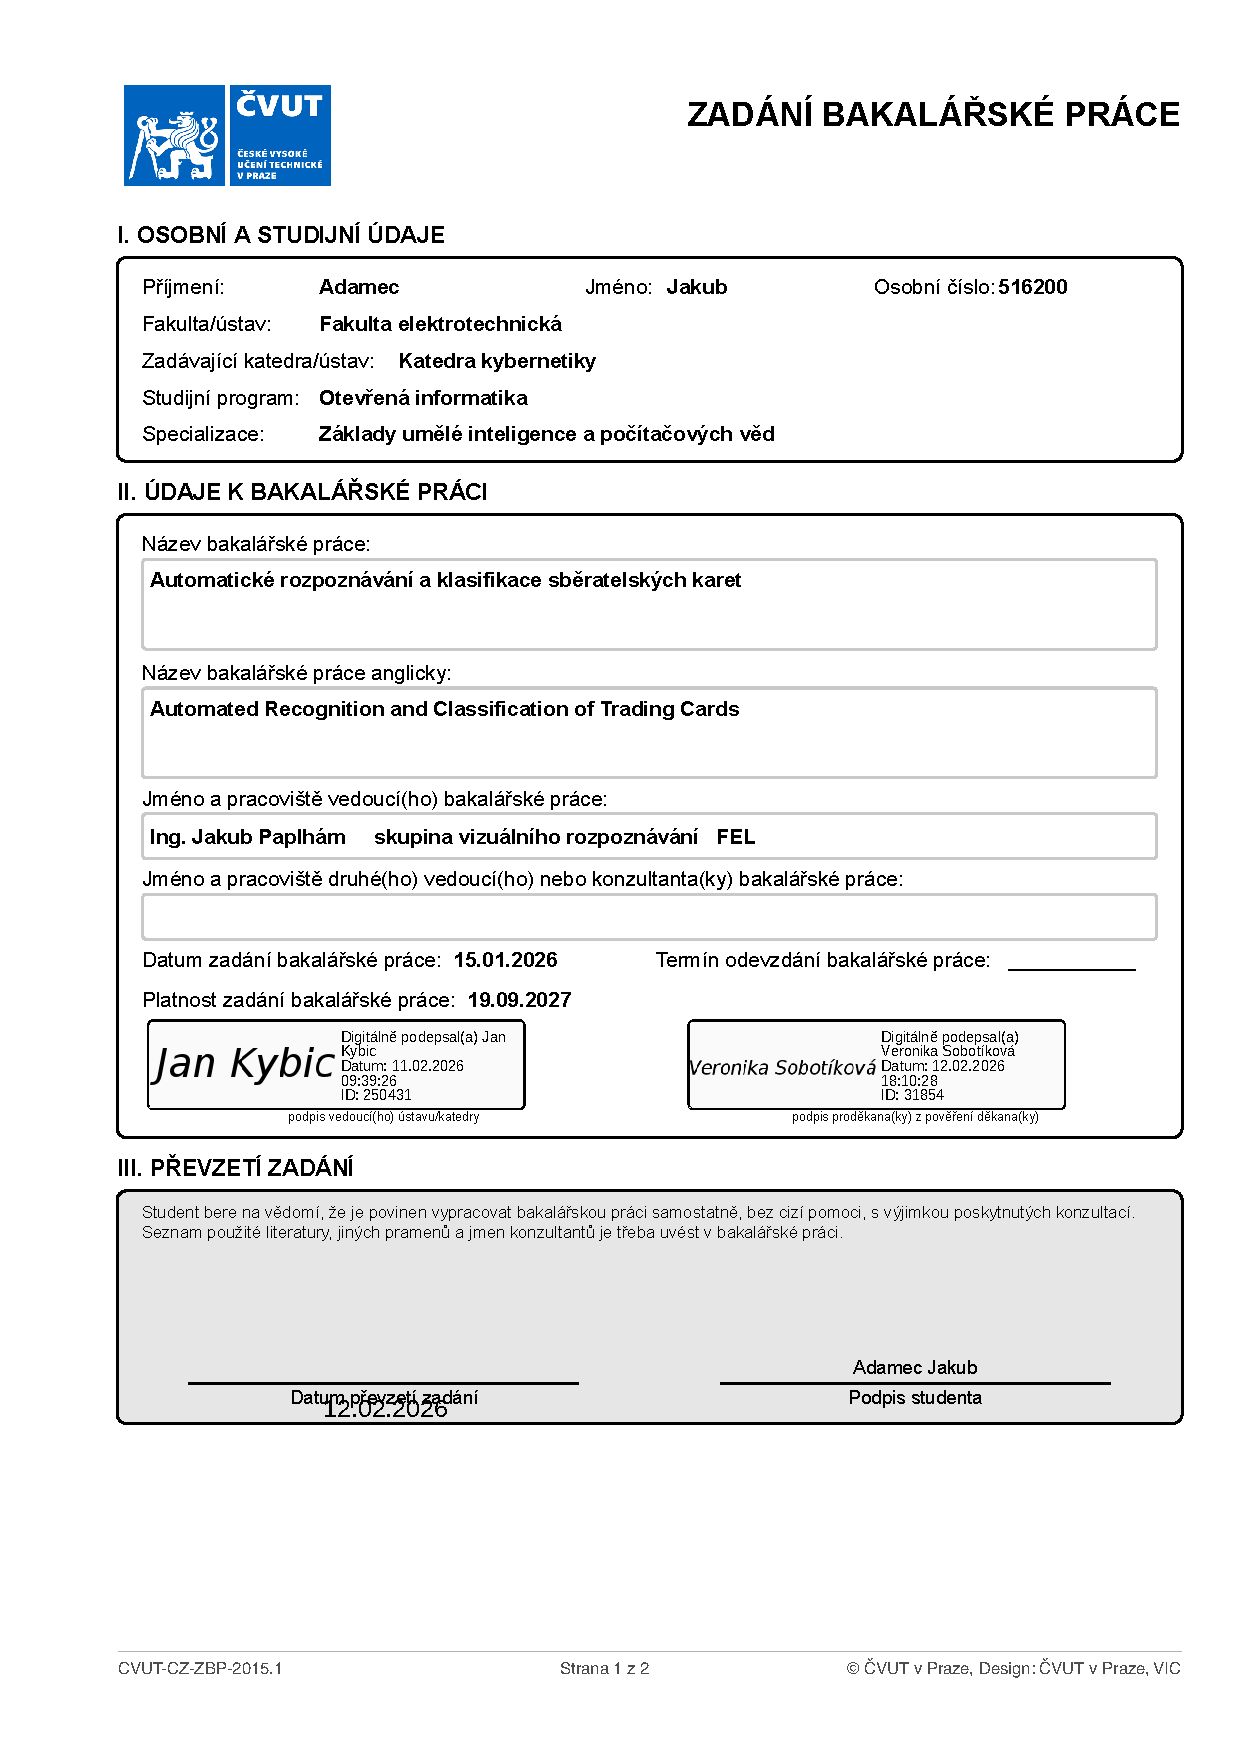
\includepdf[pages=-]{src/assignment.pdf}

%% --------------------------------------------------------------
%% |                         Declaration                        |
%% --------------------------------------------------------------

\conditionalClearPage

\input{src/declaration.tex}

%% --------------------------------------------------------------
%% |                          Abstracts                         |
%% --------------------------------------------------------------

\conditionalClearPage

%!TEX root = ../main.tex

\begin{changemargin}{0.8cm}{0.8cm}

~\vfill{}

\section*{Abstract}
\vskip 0.5em
\ac{TCG} represent a global market where the indexing and sorting of thousands of individual cards is a significant logistical challenge. As collections grow, manual sorting becomes inefficient, yet commercial automated solutions remain cost-prohibitive and rely on closed-source software ecosystems. Furthermore, traditional text-based identification methods, such as \ac{OCR}, often fail in this domain due to the prevalence of localized artistic fonts, varying languages and environmental visual noise. The primary challenge is the lack of accessible, open-source hardware and software platforms capable of robust visual card identification. Here we present an open-source robotic sorting platform integrated with a deep metric learning computer vision pipeline that identifies \ac{TCG} cards based on holistic visual similarity. By applying an \ac{arcface} to a \acs{ResNet}-50 backbone, the system mapped card artworks into a 512-dimensional Euclidean space, enabling fast vector retrieval. To overcome the absence of labeled real-world datasets, we developed a synthetic data generation pipeline that blended digital card templates onto stochastic backgrounds, simulating physical artifacts like lens glare, sensor noise and partial occlusions. This methodology effectively bridged the domain shift between digital scans and physical objects. Our experimental results demonstrated a 97.8\,\% Top-1 retrieval accuracy on unconstrained physical photographs without training on any real-world images. We anticipate this open-source architecture will serve as a baseline for accessible robotic sorting and enable the automated generation of large-scale, real-world \ac{TCG} datasets in the future.

\vskip 1em

{\bf Keywords} \Keywords

\vskip 2.5cm

\end{changemargin}


\conditionalClearPage

%!TEX root = ../main.tex

\begin{changemargin}{0.8cm}{0.8cm}

~\vfill{}

\section*{Abstrakt}
\vskip 0.5em
Sběratelské karetní hry (\ac{TCG}) představují globální trh, na kterém je indexace a třídění tisíců jednotlivých karet významnou logistickou výzvou. S rozšiřováním sbírek se ruční třídění stává neefektivním, zatímco komerční automatizovaná řešení jsou stále cenově nedostupná a spoléhají se na softwarové ekosystémy s uzavřeným zdrojovým kódem. Kromě toho tradiční textové metody identifikace, jako je optické rozpoznávání znaků (\ac{OCR}), v této oblasti často selhávají kvůli převaze lokalizovaných uměleckých fontů, různých jazyků a vizuálního šumu v okolí. Hlavní výzvou je nedostatek dostupných hardwarových a softwarových platforem s otevřeným zdrojovým kódem, které by byly schopné spolehlivé vizuální identifikace karet. Zde představujeme robotickou třídicí platformu s otevřeným zdrojovým kódem integrovanou s počítačovým zrakem využívajícím hluboké metrické učení, která identifikuje karty \ac{TCG} na základě celkové vizuální podobnosti. Aplikací Additive Angular Margin Loss (\ac{arcface}) na páteř \ac{ResNet}-50 systém zmapoval umělecká díla na kartách do 512dimenzionálního euklidovského prostoru, což umožnilo rychlé vyhledávání vektorů. Abychom překonali absenci označených datových sad z reálného světa, vyvinuli jsme proces generování syntetických dat, který míchal digitální šablony karet na stochastická pozadí a simuloval fyzické artefakty, jako je odlesk objektivu, šum senzoru a částečné zakrytí. Tato metodika účinně překlenula doménový posun mezi digitálními skeny a fyzickými objekty. Naše experimentální výsledky prokázaly 97,8\,\% přesnost vyhledávání Top-1 na neomezených fyzických fotografiích bez trénování na jakýchkoli reálných obrázcích. Předpokládáme, že tato open-source architektura poslouží jako základ pro dostupné robotické třídění a v budoucnu umožní automatizované generování rozsáhlých reálných datových sad \ac{TCG}.

\vskip 1em

{\bf Klíčová slova } \KlicovaSlova

\vskip 2.5cm

\end{changemargin}


%% --------------------------------------------------------------
%% |                        Abbreviations                       |
%% --------------------------------------------------------------

\conditionalClearPage

\begin{changemargin}{0.8cm}{0.8cm}

~\vfill{}

% \section*{Abbreviations}

\printacronyms[name=Abbreviations, heading=section*]
% this will print only the used abbreviations

\vskip 2.5cm

\end{changemargin}

\conditionalClearPage

%% --------------------------------------------------------------
%% |                      Table of contents                     |
%% --------------------------------------------------------------

\tableofcontents

\conditionalClearPage

% set up the full page style with normal page numbering
\pagestyle{full}
\pagenumbering{arabic}

%% --------------------------------------------------------------
%% |                         Main Text                          |
%% --------------------------------------------------------------

%!TEX root = ../main.tex

\chapter{Introduction}\label{chap:introduction}

\acp{TCG} such as \ac{MTG}, \ii{Pokémon}, and various sports card collections have evolved from simple hobbies into a global market with significant economic value. The secondary market for these collectibles is vast, with prices fluctuating based on card condition, rarity, and demand. For collectors and local game stores, inventory management is a critical task. This involves sorting thousands of cards, assessing their condition, and determining their current market value. However, as collections grow, manual sorting becomes an increasingly time-consuming, tedious, and error-prone process.

And if an individual, such as a collector, but also a store or company, wants to effectively index and sort cards, the current market situation offers relatively few solutions. Moreover, these solutions are often prohibitively expensive, proprietary, or cannot be customized to individual workflow needs.

\section{Problem Statement}
The primary motivation for this work is the lack of accessible, affordable, and transparent tools for automating card indexing. Existing consumer machines often fail to meet specific requirements, are unavailable in certain geographical regions, or lack the robustness needed to handle valuable collectibles without damaging them. 

\noindent
From a technical perspective, the challenge is twofold:
\begin{enumerate}[(a)]
    \item \ii{Mechanical:} Designing a sorting mechanism that handles delicate paper objects reliably without jamming or causing surface damage.
    \item \ii{Computational:} Developing a computer vision pipeline capable of fine-grained classification. Unlike standard object detection, trading cards often share identical layouts with only minor variation in artwork or text, requiring high-precision feature extraction and matching under varying lighting conditions.
\end{enumerate}

\section{Objectives}
The goal of this project is to develop an automated system for recognizing and classifying trading cards that follows the philosophy of Open-source software and hardware. By designing a robot based on accessible components, such as an Arduino microcontroller and stepper motors, and combining it with modern computer vision techniques, this work aims to democratize the technology needed for card sorting.

%%%%%% FROM MRS TEMPLATE:
\section{Thesis Contribution}


\section{Thesis Structure}


\section{Mathematical notation}
It is a good practice to define basic mathematical notation in the introduction.
See \reftab{tab:mathematical_notation} for an example.
\begin{table*}[ht!]
  \scriptsize
  \centering
  \noindent\rule{\textwidth}{0.5pt}
  \begin{tabular}{lll}
    $\mathbf{x}$, $\bm{\alpha}$ & vector, pseudo-vector, or tuple\\
    $\mathbf{\hat{x}}$, $\bm{\hat{\omega}}$& unit vector or unit pseudo-vector\\
    $\mathbf{\hat{e}}_1, \mathbf{\hat{e}}_2, \mathbf{\hat{e}}_3$ & elements of the \emph{standard basis} \\
    $\mathbf{X}, \bm{\Omega}$ & matrix \\
    $\mathbf{I}$ & identity matrix \\
    $x = \mathbf{a}^\intercal\mathbf{b}$ & inner product of $\mathbf{a}$, $\mathbf{b}$ $\in \mathbb{R}^3$\\
    $\mathbf{x} = \mathbf{a}\times\mathbf{b}$ & cross product of $\mathbf{a}$, $\mathbf{b}$ $\in \mathbb{R}^3$\\
    $\mathbf{x} = \mathbf{a}\circ\mathbf{b}$ & element-wise product of $\mathbf{a}$, $\mathbf{b}$ $\in \mathbb{R}^3$ \\
    $\mathbf{x}_{(n)}$ = $\mathbf{x}^\intercal\mathbf{\hat{e}}_n$ & $\mathrm{n}^{\mathrm{th}}$ vector element (row), $\mathbf{x}, \mathbf{e} \in \mathbb{R}^3$\\
    $\mathbf{X}_{(a,b)}$ & matrix element, (row, column)\\
    $x_{d}$ & $x_d$ is \emph{desired}, a reference\\
    $\dot{x}, \ddot{x}, \dot{\ddot{x}}$, $\ddot{\ddot{x}}$ & ${1^{\mathrm{st}}}$, ${2^{\mathrm{nd}}}$, ${3^{\mathrm{rd}}}$, and ${4^{\mathrm{th}}}$ time derivative of $x$\\
    $x_{[n]}$ & $x$ at the sample $n$ \\
    $\mathbf{A}, \mathbf{B}, \mathbf{x}$ & LTI system matrix, input matrix and input vector\\
    \emph{SO(3)} & 3D special orthogonal group of rotations\\
    \emph{SE(3)} & \emph{SO(3)}~$\times~\mathbb{R}^3$, special Euclidean group\\
  \end{tabular}
  \noindent\rule{\textwidth}{0.5pt}
  \caption{Mathematical notation, nomenclature and notable symbols.}
  \label{tab:mathematical_notation}
\end{table*}

\chapter{Related Work}\label{chap:rw}

The automation of trading card sorting is a multi-disciplinary problem intersecting mechanical engineering, robotics, and computer vision. While the market for \acp{TCG} has existed for decades, automated solutions have only recently become viable due to advancements in deep learning and affordable rapid prototyping tools. This chapter reviews existing commercial systems and relevant academic literature, categorizing them into mechanical handling solutions and algorithmic recognition strategies.

\section{Commercial Solutions}
The current market for automated sorting is dominated by high-cost, closed-source proprietary systems. These machines are typically designed for high-volume businesses rather than individual collectors.

\subsection{Hardware-Based Sorters}
\begin{itemize}
    \item \bb{\ac{TCG} Machines:} The \ii{PhyzBatch-9000} by \ii{\ac{TCG} Machines} \cite{tcgmachines} represents the industrial standard. It addresses a specific computer vision challenge: holographic glare. By utilizing specialized LED arrays and diffusers, the machine controls lighting conditions to detect \enquote{foil} (holographic) cards, which are prone to over-exposure in standard camera setups.
    \item \bb{CardBot:} \ii{CardBot} \cite{cardbot} differs in its handling mechanism. Unlike friction-based feeders, which can scratch the surface of cards, \ii{CardBot} uses a pneumatic suction system. This approach minimizes physical contact with the card surface, which is essential to prevent damage to the cards.
    \item \bb{Magic Sorter:} \ii{Magic Sorter} \cite{magicsorter} offers a more compact alternative, focusing specifically on \ii{Magic: The Gathering} cards. It integrates a feeder mechanism with a custom software suite, demonstrating the tight coupling between hardware and proprietary databases common in commercial tools.
\end{itemize}

\subsection{Software Ecosystems}
Apart from hardware, pure software solutions attempt to streamline the cataloging process. \ii{Card Dealer Pro} \cite{carddealerpro} provides a computer-vision-based inventory management system. While effective, such solutions rely on the user to manually present cards to a webcam or scanner, lacking the robotic automation required for bulk processing.

\section{Algorithmic Approaches to Recognition}
The core challenge in automating \ac{TCG} sorting is the reliable identification of card artwork among tens of thousands of similar classes. Research in this domain generally falls into two categories: \ac{OCR} and \ac{VSL}.

% \subsection{OCR and Text-Based Identification}
% A traditional approach involves reading the card's title and set code. A case study by \ii{Oodles Technologies} for \ii{Erie \ac{TCG}} \cite{erietcg} explored this using \ac{NER} and \ac{OCR}. 

% While theoretically sound, this approach struggles in practice due to the \enquote{artistic} nature of \acp{TCG}. Text is often stylized, obscured by artwork elements, or printed on holographic backgrounds that confuse standard \ac{OCR} engines. Consequently, text extraction is often computationally expensive and brittle compared to visual matching.

\subsection{Visual Similarity and Metric Learning}
Modern approaches favor deep learning techniques that treat the card as a holistic visual fingerprint rather than a text document.

\subsubsection{Siamese Networks}
Lowhur \cite{lowhuryugioh} demonstrated a highly effective system for \ii{Yu-Gi-Oh!} cards achieving 99\% accuracy. The methodology moves away from standard classification (which requires retraining for every new card set) to \ii{Metric Learning}. 

By utilizing Siamese Networks and triplet loss functions, the model learns an embedding space where images of the same card are clustered together. This allows the system to identifying cards by comparing their feature vectors against a database, a technique known as \ii{One-Shot Learning}.

\subsection{Object Detection and Robotics Integration}
Recent academic work has focused on the pipeline of locating objects (detection) and manipulating them (robotics).

\subsubsection{YOLO for Real-Time Detection}
The \ac{YOLO} architecture is the standard for real-time localization.
\begin{itemize}
    \item \bb{Robotic Integration:} Yu \cite{pokerrobot} validated the integration of vision and pneumatics in a self-playing poker robot. The study successfully combined \ac{YOLO}v5 for card localization with a suction-cup robotic arm. This provides a direct precedent for the hardware-software integration proposed in this thesis, confirming that suction mechanisms are viable for thin card stock.
    \item \bb{Pipeline Validation:} Freitter \cite{idcardverification} proposes a pipeline for ID card verification that mirrors the requirements of \ac{TCG} sorting: segmentation using \ac{YOLO}v8 followed by classification using \ac{ResNet}. This \enquote{two-stage} approach: first finding the object, then identifying it; is robust against background noise and variable lighting.
\end{itemize}

\subsubsection{The Data Scarcity Problem}
A major hurdle in training neural networks for TCGs is the lack of labeled training data for the millions of unique cards in circulation. Pua \cite{pokemonstanford} addressed this in a study on \ii{Pokémon} card detection. Instead of manually photographing thousands of cards, the authors developed a \bb{Synthetic Data Generation} pipeline. By projecting digital card scans onto varying backgrounds and applying simulated lighting, noise, and occlusions, they successfully trained a robust \ac{YOLO}v8 model. This methodology highlights that synthetic data is not only a time-saver but a necessity for achieving high robustness in \ac{TCG} recognition.

\section{Summary}
Current commercial solutions like \ii{CardBot} provide robust hardware but remain inaccessible due to cost and closed ecosystems. Conversely, academic research provides individual building blocks: \ac{YOLO} for detection \cite{pokerrobot}, synthetic data for training \cite{pokemonstanford}, and Siamese networks for identification \cite{lowhuryugioh}. But rarely integrates them into a complete, open-source device. This thesis aims to bridge this gap by combining these state-of-the-art algorithmic techniques with a low-cost, replicable hardware design.
\chapter{Hardware Design}\label{chap:hw}
The design of the robotic system focuses on accessibility, replicability, and gentle handling of the trading cards. 
This system utilizes a vacuum-based pick-and-place mechanism. This chapter details the component selection, the 
pneumatic subsystem, circuit design, and the mechanical construction.

\section{Component Selection} % TODO
The selection of components was driven by the availability of parts on the consumer market and the cost-to-performance 
ratio. A summary of key components is provided in 
\reftab{tab:components}.
\begin{table}[!h]
    \centering
    \caption{List of key hardware components.}
    \label{tab:components}
    \begin{tabular}{l|l|l}
        \textbf{Component} & \textbf{Model/Type} & \textbf{Primary Function} \\ \hline
        Microcontroller & Arduino Mega 2560 & Main control unit \\
        Stepper motor & & \\
        Stepper motor driver & TMC2209 & \\
        Rotary position sensor & AS5147-TS\_EK\_AB & Rotation feedback \\
        Servo motor & MG90s & \\
        Compressor & Sparmax TC-610H Plus & Air pressure source \\
        Venturi generator & custom 3D print & Vacuum generator \\
        Suction cup & SB 15,5 mm silicon, bellows & Card handling \\
        Pneumatic valve & Solenoid valve G356NC-18B & Controlling the airflow \\
        Noise suppressor & AE-M5 & Noise reduction \\
        Air hoses & Polyuretan, 6/4 mm & 
    \end{tabular}
\end{table}

\subsection{Control Electronics}

\subsubsection{Microcontroller: Arduino Mega}
The \textit{Arduino Mega 2560} was selected as the central processing unit. Although modern 32-bit boards (like ESP32) 
offer more power, the Mega provides a high number of GPIO pins (54 digital), which allows for easy expansion without 
multiplexing. Its 5 V logic level simplifies interfacing with certain industrial sensors, and its vast community support 
aligns with the project's educational goals.

\subsubsection{Stepper Motor and Driver}
A standard stepper motor combined with a \textit{TMC2209} driver from Trinamic is used to move the robotic arm. 
The \textit{TMC2209} driver allows configuration of motor current and micro-steps via UART, eliminating the need to work 
with a potentiometer directly on the driver. 

\subsubsection{Feedback Loop: AS5147 Encoder}
To ensure precise positioning, the system is equipped with an \textit{AS5147} magnetic rotary encoder. This sensor 
communicates via SPI and provides absolute angular position. By combining the stepper motor with this encoder, the 
system operates in a closed-loop manner, allowing it to detect missed steps or jams, which is critical for preventing 
damage to valuable cards.

\subsection{Pneumatic System}

Handling trading cards mechanically (e.g., with rubber rollers) carries a risk of scratching surfaces or bending 
corners. Therefore, a pneumatic vacuum system was designed to lift cards from the top.

\subsubsection{Air Source: Sparmax TC-610H Plus} % TODO:

\subsubsection{Vacuum Generation and Handling}
Since the compressor generates positive pressure, a \textit{Venturi generator} is used to convert compressed air into a 
vacuum. A \textit{3/2-way solenoid valve} (24 V DC, Normally Closed) controls the airflow. The 3/2 configuration is 
essential: in the \enquote{off} state, it not only stops the supply but also vents the vacuum line to the atmosphere,
allowing the card to drop instantly. Silicone suction cups with bellows are used to transfer contact with the cards 
themselves. Silicone was chosen for its softness and adhesion. Bellows were chosen to help compensate for imperfections 
in the contact between the arm and the card.

% \includesvg[inkscapeformat=pdf]{fig/sketch/magstep.svg}

\includepdf{fig/sketch/output.pdf}
\chapter{Methodology}\label{chap:me}
\section{Software}\label{sec:sw}
\section{Visual Recognition}\label{sec:rec}
\input{src/chapters/07_experimentsAndResults.tex}
\input{src/chapters/08_discussion.tex}

%!TEX root = ../main.tex

\chapter{Conclusion}\label{chap:conclusion}

\section{Summary of Results}
The objective of this thesis was to design, build and evaluate an automated, open-source system for the recognition and physical sorting of trading cards. By combining accessible rapid prototyping hardware with a deep metric learning computer vision pipeline, the project demonstrated that automated \ac{TCG} cataloging can be achieved without relying on expensive, proprietary commercial solutions.

From a hardware perspective, the integration of a 3D-printed robotic manipulator with a pneumatic vacuum end-effector successfully provided a reliable, non-destructive method for handling thin paper stock. The separation of computational loads (delegating real-time motor control to an Arduino and high-level inference to a Raspberry Pi) ensured stable kinematic execution while processing image data.

On the software front, the system bypassed the inherent limitations of \ac{OCR} by treating cards as holistic visual fingerprints. Because labeled real-world datasets of the required magnitude do not exist, the network was trained entirely on digitally synthesized data. By projecting clean digital scans onto stochastic backgrounds and applying severe geometric and optical augmentations, the model was forced to learn robust feature representations. The application of the  objective function successfully structured the 512-dimensional embedding space, minimizing intra-class variance while maximizing inter-class separability.

Experimental evaluation validated this approach. The model achieved a 97.8\,\% Top-1 Name Match retrieval accuracy on a dataset of unconstrained physical photographs. The close correlation between the validation loss on synthetic data and the real-world retrieval accuracy confirmed that the proposed synthetic augmentation pipeline effectively bridged the domain shift between digital templates and physical assets.

\section{Limitations and Future Work}
While the initial prototype successfully established a baseline for open-source card sorting, several architectural components can be optimized in future iterations.

\subsection{Hardware Optimization}
The current low-level control relies on an Arduino Uno. While adequate for proving the mechanical concept, it is architecturally outdated. Future hardware iterations should replace the Arduino with modern microcontrollers from the ESP family (e.g., ESP32). ESP microcontrollers operate at higher clock speeds, offer built-in wireless connectivity (Wi-Fi and Bluetooth) and feature a significantly smaller physical footprint, often at a lower unit cost. Transitioning to an ESP32 would enable wireless control interfaces and eliminate the need for a physical serial tether between the control board and the single-board computer.

\subsection{Robust Image Localization}
The current image preprocessing pipeline uses a deterministic OpenCV algorithm (Canny edge detection coupled with morphological closing) to extract the card's bounding box from the raw camera frame. While functional in a controlled environment, this rigid algorithmic approach is sensitive to background clutter and severe specular reflections caused by glossy card sleeves. 

A more robust solution would be to replace this classical pipeline with a lightweight object detection model, such as YOLOv8 Nano~\cite{redmon2016yolo}. By training a small YOLO model specifically on the binary task of segmenting the card boundary from the background, the system could extract the homography points much more reliably across varied lighting conditions, offloading the localization logic entirely to learned features.

\subsection{Fine-Grained Edition Matching}
As discussed in \Cref{chap:er}, while the global feature extractor is highly accurate at identifying the canonical name of a card, its accuracy drops when distinguishing between visually identical reprints (Exact Edition matching). Global metric learning prioritizes macro-level artwork over micro-level typography. 

To resolve this, future work should implement a two-stage recognition architecture. The current metric learning model would serve as the primary retrieval mechanism to identify the card's name. A secondary, highly localized classification head could then be deployed to inspect specific regions of interest (such as set symbols or copyright dates) to verify the exact edition. 

Finally, the completed robotic platform can now function as an automated data acquisition tool. By processing bulk collections and utilizing the current network for pseudo-labeling, the robot can rapidly generate a large-scale dataset of real-world physical photographs. This dataset can subsequently be used to fine-tune future recognition models, entirely eliminating the reliance on synthetic data.


%% --------------------------------------------------------------
%% |                         References                         |
%% --------------------------------------------------------------

\chapter{References}

\printbibliography[heading=none,title={}]

%% --------------------------------------------------------------
%% |                         Appendices                         |
%% --------------------------------------------------------------

\appendix
\renewcommand\chaptername{Appendix}

\renewcommand{\thechapter}{A}
\renewcommand\chaptername{Appendix A}

\chapter{Appendix A}

\end{document}
